\documentclass[main.tex]{subfiles}
\begin{document}

\chapter{組合}
組合數學是一門研究可數或離散對象的數學,也就是如何數可以一個一個數的東西。競程裡面大部分的東西都是離散的,而許多動態規劃和資料結構題目都需要一些組合技巧,因此組合在競程的數學題裡面是十分重要的一部分。

\section{基本計數原則}

\subsection{簡單的問題}
有1元、2元、4元、8元硬幣任意多個,有多少種方法湊成20元?兩種方法視為不同,代表有至少一種幣值使用的硬幣個數不同。

用手算一下的話,可以發現答案為56種。雖然這個問題非常簡單,解答的過程中或許會不經意使用到核心的計數原則!
\subsection{加法原理}
假設有 \(k\)個集合 \(A_1, A_2, ..., A_k\),任兩個集合皆互斥,則
\[|\cup_{i=1}^k A_i | = \sum_{i=1}^k |A_i|\]

用白話講的話,當你要數符合某個條件的東西時,可以試著把它分成一些\textbf{互斥的情況},把每種情況的方法數加起來得到答案。
以剛剛的問題為例,我們可以將每一種方法依照「8元硬幣個數」分類,剩下只需討論使用1、2、4元三種硬幣的情況,最後再將各方法數相加即可。只不過這樣做的話還是稍嫌麻煩,於是我們用到第二個計數原理。

\newpage
\subsection{乘法原理}
假設有 \(k\)個集合 \(A_1, A_2, ..., A_k\),定義他們的笛卡爾積(Cartesian Product) 為集合
\(\Pi A_i = A_1 \times A_2 \times ... \times A_k = \{(a_1, a_2, ..., a_k) | a_i \in A_i, i = 1, 2, ..., k\}\)
則\[|\Pi A_i| = |A_1| \times |A_2| \times ... \times |A_k| = \Pi |A_i|\]

也就是說,假設每個集合都有\(c_i\)個東西可以選,那從每個集合各選一個東西有\(\Pi c_i\)種選法。\\

在剛剛的問題中,如果只考慮$1, 2$兩種硬幣,則可以發現湊出$k$元的方式有$\lfloor \frac{k}{2}\rfloor+1$種方法,那麼我們利用加法原理,枚舉4元和8元能湊出的數值(假設是$x$元),再將此方法數乘上$\lfloor \frac{20 - x}{2}\rfloor+1$就可以快速算出答案。

這兩個原理看似簡單,但幾乎所有的組合公式都是由此推導而來。


\section{排列數與組合數}
這個部分大多屬於高中數學的範圍,因此這裡會快速帶過。

\definition{組合數定義}{
\begin{itemize}
\item 階乘(factorial):$n! = \Pi_{k=1}^n k = 1 \cdot 2 \cdots n-1 \cdot n$,額外定義$0! = 1$。
\item 排列數(permutation): $P_k^n = \frac{n!}{(n-k)!}$
\item 組合數(combination): $C_k^n = \binom{n}{k} =  \frac{n!}{(n-k)!k!}$,若$k>n$或$k<0$,則定義$C_k^n = 0$。
\item 重複組合數(combination with repetitions): $H_k^n = C_{n-1}^{n+k-1}$
\end{itemize}}
\par 這些符號都有相對應的組合意義。比較不熟悉的可能是重複組合數$H_k^n$的計算方式。這個符號代表從$n$種東西中選出$k$個的組合數(每個東西可以重複任意多次)。可以把它看成是有$k$顆球與$n-1$個隔板,球跟隔板之間的每個排列方式都一一對應到重覆組合的方法,因此總方法數為$C_{n-1}^{n+k-1}$。

\subsection{如何計算組合數}
競程裡的組合題目通常會要求輸出方法數模一個大質數的結果(如$10^9 + 7$或$998244353$)。因此以下皆討論$mod \ p$時的狀況。
\newpage
\begin{center} 用階乘的定義算 \end{center}
\begin{C++}
#define ll long long
const int mod = 1e9 + 7;
const int maxn = 100005;
ll modpow(ll a, ll p) {}//快速冪略
ll fac[maxn], finv[maxn]; //階乘與階乘的模反元素
ll C(int n, int m){
    if (m > n) return 0;
    return fac[n] * finv[m]%mod * finv[n-m]%mod;
}
int main() {
    fac[0] = finv[0] = 1;
    for (int i = 1;i < maxn;i++) {
        fac[i] = fac[i-1] * i %mod;
        finv[i] = modpow(fac[i], mod - 2); //費馬小定理
    }
}
\end{C++}
此方法需要$O(n)$預處理時間,可以$O(1)$算出$C(n, m)$的值,其中$n$是題目最大需要的數值。

\begin{center} 巴斯卡三角形 \end{center}
\begin{C++}
ll c[maxn][maxn];
int main() {
    c[0][0] = 1;
    for (int i = 1;i < maxn;i++) {
        for (int j = 0;j <= i;j++) {
            c[i][j] = (c[i-1][j] + 
            (j ? c[i-1][j-1] : 0))%mod;
        }
    }
}
\end{C++}
此方法需要$O(n^2)$預處理時間,$O(1)$查詢時間,當$n$不大時,計算時間會較低。\\

另外,當模數不大時,可以用\href{https://en.wikipedia.org/wiki/Lucas\%27s_theorem}{Lucas's Theorem}求組合數,當$\binom{n}{k}$中的$k$不大時可以直接用乘的算出答案,另外有許多求組合數的方法,有興趣的讀者可以自行查資料。

\section{組合公式}
以下是許多組合計數中經常使用的公式,適當的使用往往能降低計算的複雜度。

\lemma{組合恆等式}{
\begin{itemize}
    \item 對稱性: \(\binom{n}{k} = \binom{n}{n-k}\)
    \item 巴斯卡定理: \(\binom{n}{k} + \binom{n}{k+1} = \binom{n+1}{k+1}\)
    \item 二項式定理: \((x+y)^n = \sum_{k=0}^n \binom{n}{k} x^k y^{n-k}\)
\end{itemize}
}
這些組合恆等式可以用代數的方法證明,也可以使用組合證明(Combinatorial Proof)解釋。組合證明的好處是相對直觀,而能夠說明該公式實際的意義。以下面的問題為例:
\problem{范德蒙恆等式 Vandermonde's Identity}{
試用組合的方式證明 \[\sum_{i=0}^{k} \binom{n}{i} \binom {m}{k-i} = \binom{n+m}{k}\]
}
解答: 考慮從$n$個男生和$m$個女生中選出$k$個人,顯然有$\binom{n+m}{k}$種選法,而假設固定選了$i$個男生,會有$\binom{n}{i}\binom{m}{k-i}$種方法,因此根據加法原則,選$0$到$k$個男生的總方法數和必為$\binom{n+m}{k}$。
\par 上述的證明為「數兩次」證明法的一個例子,用兩種方法計算同一個東西的方法數,藉此證明兩種方法的公式得到的結果相等。\\
接下來用一個例子介紹另外一種組合證明。

\subsection{卡特蘭數}
\problem{一路領先問題}{
以下各種問題都互相等價:
\begin{itemize}
    \item $n$個左括弧和$n$個右括弧組成合法括號字串的方法數。
    \item 在$n \times n$的方格中從左下角的格子點走捷徑到右上角,且不經過左下-右上對角線(即$x=y$)的方法數。
    \item $n+1$個葉節點的完全二元樹個數。
\end{itemize}
這些問題的方法數都相同,我們稱之為第$n$個卡特蘭數(Catalan Number) $C_n$
}
以第一個問題來說,應該有些人最先想到的是用動態規劃來解這題,令$dp_{i, j}$代表前$i$個字元中\textbf{\('('\text{的個數} - ')'\text{的個數為}j\)}的方法數。則有以下轉移式:
\[dp_{i, j} = 
\begin{cases}
dp_{i-1, j-1} + dp_{i-1, j+1}, & \text{if}\ j \geq 0 \\
0, & \text{otherwise}
\end{cases}\],最後答案為$dp_{2n, 0}$。這樣的複雜度為$O(n^2)$,但我們能做到更好! 
\\
\par 考慮第二種問題(在格子走捷徑),以下用「路徑」簡稱任意一條由左下至右上的路徑。我們想要證明$C_n = \binom{2n}{n} - \binom{2n}{n-1}$,但首先需要先介紹一些名詞。
\definition{函數的類別}{
數學中的函數$f: A \rightarrow B$可以想成是兩個集合$A, B$之間的對應關係,其中:
\begin{itemize}
\item 單射(injective)函數: 每個$A$的元素都對應到一個$B$的元素。且$A$內相異元素對應到的值皆不同。
\item 滿射(surjective)函數: 每個$B$的元素都有至少一個$A$的元素對應到。
\item 雙射(bijective)函數: 每個$A$的元素都一一對應到$B$的元素。函數為雙射若且唯若同時是單射跟滿射。
\end{itemize}
}
接下來使用的組合證明法稱為雙射原則(bijection principle)。
\lemma{雙射原則}{
若有兩個可數的集合$A, B$之間可以建立雙射函數,則$|A| = |B|$。
}
回到卡特蘭數的證明。左邊的$\binom{2n}{n}$顯然是在沒有限制下的路徑方法數,因此可以猜測扣掉的$\binom{2n}{n-1}$代表「不合法的路徑數」。我們將在$(n-1)\times(n+1)$的路徑與$n\times n$格子內不合法的路徑之間建立雙射。\\ \\
考慮以下兩張圖: \\ 
\begin{center}
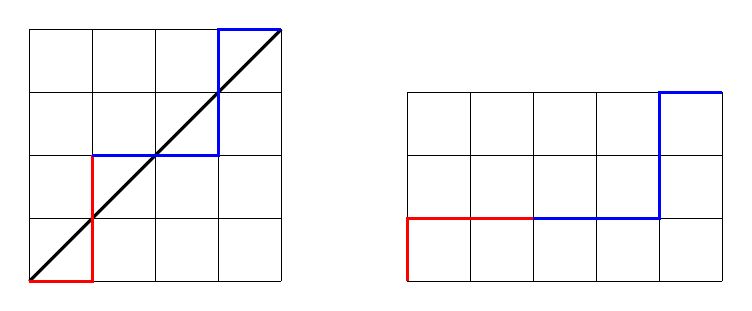
\begin{tikzpicture}[scale=0.8,]
 \draw[step=1.0,black,thin] (0.0,0.0) grid (4.0,4.0);
\draw [black, very thick] (0, 0) -- (4, 4);
\draw [red, very thick] (0, 0) -- (1, 0) -- (1, 2);
\draw [blue, very thick] (1, 2) -- (3, 2) -- (3, 4) -- (4, 4);
\draw[step=1.0,black,thin] (6.0,0.0) grid (11.0,3.0);
\draw [red, very thick] (6, 0) -- (6, 1) -- (8, 1);
\draw [blue, very thick] (8, 1) -- (10, 1) -- (10, 3) -- (11, 3);
\end{tikzpicture}
\end{center}
對於任意一條不合法的路徑,都可以找到第一次跨越對角線的地方(左圖的紅色線段),此時往上步數$=$往右步數$+1$。將紅色線段依對角線翻轉,後面再接上藍色線段,就可以得到一條在$(n-1)\times(n+1)$方格的路徑。不難證明這個轉換會建立雙射,而右邊方格的路徑數為$\binom{2n}{n-1}$,故根據雙射原則,不合法的路徑數亦為$\binom{2n}{n-1}$,上述公式因此得證,我們就能在$O(n)$時間找到$C_n$的值。

卡特蘭數還有兩個遞迴式跟其他性質,有興趣的讀者可以參考\textbf{\href{https://en.wikipedia.org/wiki/Catalan_number}{維基百科}}。

\section{鴿籠原理}
\theorem{鴿籠原理}{
假設有$n$個物品要分成$k$堆,東西最少的一堆數量$\leq \lfloor \frac{n}{k} \rfloor$,東西最多的一堆數量$\geq \lceil \frac{n}{k} \rceil$
}
這個定理常常出現在一些存在性證明裡面用到,在競程裡也可以用來尋找上下界。
\problem{怪怪背包?}{
給定$n$個的整數,證明一定存在一個非空子集使得總和為$n$的倍數。
}
\newpage
這類證明的問題要做的事就是找到「物品」跟「箱子」。總和為$n$的倍數,也相當是總和模$n$為$0$,那我們就把總和模$n$的值視為箱子吧!任意排序這$n$個整數並計算他們的前綴和模$n$並放進箱子,如果有一項放進$0$的箱子的話就有解了,否則只有$n-1$個箱子可以放,必定存在一個箱子有兩個東西,此時取這兩個前綴相減的區間就能得到總和為$n$的倍數的子集。


\section{使用動態規劃}
程式競賽中最常使用到排組的地方就是動態規劃問題了,先看看一個例題:
\problem{\href{https://tioj.ck.tp.edu.tw/problems/1291}{N 箱 M 球}}{
$n$個相同的箱子要放入$m$個不同的球,問有幾種放法。輸出方法數$\mod 10^6$的結果。\\
$n, m \leq 200$,有多筆測資。
}
這裡提供兩種解法,兩種都需要對不同的方法進行分類。 \\
因為$m$顆球皆相異,我們可以把球編號$1, 2, \dots m$。而$n$個箱子相同,因此他們放在一排之後任意排序都會是一樣的方法,而箱子內的球也是無序的。 \\

解一: 考慮$1$號球所在的箱子,我們可以把所有分法依照這個箱子有多少顆球分類。令$dp_{i, j}$代表$i$個箱子放$j$顆球的方法數。若$j = 0, dp_{i, j} = 1$。假設$1$號球所在箱子有$k$顆球,剩下$k-1$顆球有$\binom{j-1}{k-1}$種選法,而之後剩$j-k$顆球放在$i-1$個箱子。故轉移式為:$dp_{i, j} = \sum_{k=1}^j \binom{j-1}{k-1} dp_{i-1, j-k}$,初始條件$dp_{0, 0} = 1$。時間複雜度為$O(nm^2)$。\\

解二: 令$dp_{i, j}$代表$i$個箱子放$j$顆球,且\textbf{每個箱子都至少有一顆球}的方法數。考慮$1$號球所在箱子,如果箱子只有$1$號球的話,剩下球有$dp_{i-1, j-1}$種放法。否則,在放$1$號球之前每個箱子至少有一顆,對於所有$dp_{i, j-1}$種方法,$1$號球都能放在$i$個箱子中任意一個。因此有轉移式:$dp_{i, j} = dp_{i-1, j-1} + i * dp_{i, j-1}$。初始條件$dp_{0, 0} = 1$。最終的答案為$\sum_{k \leq n} dp_{k, m}$,時間複雜度$O(nm)$。 \\

由上面的問題可以發現,有一些組合問題不一定有一個乾淨的解析解(closed form),但在題目限制下好好使用遞迴就能解決許多問題!
\newpage
\section{機率與期望值}
\definition{期望值}{
一個隨機變數$X$有$n$種可能的事件,第$i$個事件價值是$v_i$,發生的機率是$p_i$,且$\sum_{i=1}^n p_i = 1$,那麼這個隨機變數的期望值$E(X) = \sum v_i p_i$
}
期望值的問題可以有許多變化,因為他其實只是「求和問題」的一種變形而已。而這個時候會運用到一個非常重要的性質。
\lemma{期望值的疊加性(linearity of expectation)}{
\[E(X_1 + \dots X_n) = E(X_1) + E(X_2) + \dots + E(X_n)\]
}
這個性質告訴我們,如果可以把一個事件拆成一些互不影響(獨立)的小事件,並且能算出小事件的價值跟機率的話,就可以枚舉小事件把期望值相加! 來看一個實際的例子。
\problem{\href{https://tioj.ck.tp.edu.tw/problems/2163}{神奇寶貝獎章 (TIOJ 2163)}}{
星街跟姐街在玩一個遊戲,星街有$n$張牌,每張牌上面數字分別為$a_1, a_2, \dots, a_n$,姐街有$m$張牌,上面數字為$b_1, b_2, \dots, b_m$,且這$n+m$張牌數字兩兩相異。兩人各隨機選$k$張牌,由小到大排好後比大小,第$i$張牌數字較大者得一分。星街想知道,她期望得分是多少?假設答案化為最簡分數是$\frac{P}{Q}$,輸出$PQ^{-1} \mod 998244353$。
$1 \leq k \leq n, m \leq 500$
}
顯然,直接枚舉所有$\binom{n}{k} \binom{m}{k}$種組合會太慢,這時候就可以用前面的性質。在比大小的時候,假設第$i$個位置是比較$a_x, b_y$,我們就可以算出它的價值(得分),至於發生的機率,星街需要在前$x-1$項選$i-1$項,在後$n-x$項選$k-i$項。姐街那邊也一樣,所以方法數有$\binom{x-1}{i-1} \binom{n-x}{k-i} \binom{y-1}{i-1} \binom{m - y}{k-i}$種!把這個總和算出來,最後除以$\binom{n}{k} \binom{m}{k}$就可以得到答案。
\subsection{遞迴關係}
\par 另外,有一種類型的問題是要問你某件事情發生前的步數,但這個步數可能是無限的,以下面的例題來說:
\problem{幾何分佈}{
骰一顆六面骰直到出現$6$為止,期望要幾次?
}
\par 數學好的人可能會列出一個無窮等比級數的算式得到答案,但其實有另一種方法。假設答案是$E$,那麼可以列出遞迴式$E = 1 + \frac{5}{6}E$, 輕鬆得到正確答案$E = 6$。\textbf{這裡預先假設了答案會收斂,數學考試別這樣寫},但是上述的方法對一些更複雜的期望值題目比較有用。有一種題目是要將每一種狀態視為一個變數,狀態之間的轉移是一個方程式,最後再用高斯消去(或是其他技巧)解開一組方程式。

\section{排容原理}
高中課程裡提到了兩項與三項的排容原理,但在競賽程式中,更常用到的是推廣的版本,先來看看排容原理本身的敘述:
\theorem{排容原理}{
有$n$個集合$S = \{A_1, A_2, \dots, A_n\}$,宇集為$U$, 令$T \in S$,$F(T)$為集合$T_1 \cap \dots T_k$的大小,則\[|U \setminus \cup_{i=1}^n A_i | = \sum_{T \in S} (-1)^{|T|}F(T)\]
如果$F(T)$的值只跟$T$的大小有關(用$f(|T|)$表示,那也可以寫成 \[|U \setminus \cup_{i=1}^n A_i | = \sum_{k=0}^n (-1)^{k}\binom{n}{k}f(k)\]
}
證明:考慮任何一個元素$x$,假設它在一些集合$A_{i_1}, \dots, A_{i_k}, k \neq 0$裡面,則$x$在左式貢獻的數量為$0$,在右式貢獻$\binom{k}{0} - \binom{k}{1} + \dots + (-1)^{k}\binom{k}{k} = 0$,否則,$x$在左式貢獻為$1$,右式貢獻也是$\binom{0}{0} = 1$,故得證。
\\
\par 可以注意到:排容原理是加法原理的延伸,而許多數個數的問題都需要扣除重複的情況,因此我們可以利用排容原理,計算出右式的結果。一個思考排容問題的訣竅是:把集合視為某種條件,那麼要算「不符合所有條件」的數量就能用「符合$x$個條件的個數」算出。
以錯排問題為例:
\problem{錯排數}{
給定$n$,數有多少個$1, \dots, n$的排列沒有任何定點,即不存在$1 \leq i \leq n$使$a_i = i$。
}
令第$i$個條件是$a_i = i$,則答案為符合$0$個條件的排列數。可以知道,不符合$x$個條件$a_{i_1} \dots a_{i_x}$的排列數有$(n-x)!$個,而這個值只跟$x$有關,因此$f(x) = (n-x)!$, 答案為$\sum_{i=0}^n (-1)^i \binom{n}{i}(n-i)!$。\\

以下來看一題比較難的問題。
\problem{$k$逆序數對排列計數}{
給定$n, k$, 數有多少個$1, \dots, n$的排列有恰$k$個逆序數對。$n \leq 10^5, k \leq min(\binom{n}{2}, 10^5)$
}
首先,問題可以轉換為:數有多少個序列$a_1, \dots, a_n$使得$0 \leq a_i < i$且$\sum a_i = k$ (轉換方式留給讀者練習)。這裡有一個顯然的$O(n^2)$背包做法,但要怎麼樣更快呢?
\par 我們令第$i$個條件是$a_i \geq i$,那麼答案會是符合$0$個條件的序列數。在沒有條件限制下,總和為$k$的方法數為$H_k^n = \binom{n-1+k}{n-1}$。有條件限制時,我們需要找到類似的方法計算答案。問題是,假設我們枚舉不符合$x$個條件的個數的話,這個方法數還會跟那個集合$T$內的元素有關!
\par 那樣是不是就沒救了?其實不一定。仔細觀察會發現,我們如果知道$T$內元素總和是$s$,那$F(T) = \binom{n-1+k-s}{n-1}$,把式子寫開來會得到:
\[\textbf{答案} = \sum_{i=0}^n (-1)^{i} \sum_{s=0}^k\binom{n-1+k-s}{n-1} g(s, i) \]
其中$g(s, i)$代表有多少種方法用$i$個相異且$\leq n$的正整數湊出$s$。這樣寫出來有什麼好處呢?可以發現因為所有數字必須相異,$i$個相異正整數最小總和是$\frac{i(i+1)}{2}$,所以$i$的範圍只會到$O(\sqrt(k)$,狀態數就是$O(k\sqrt k)$!最後,$g(s, i)$可以用前面提到的dp技巧計算出來,留給讀者練習。





\newpage
\section{例題}
\problem{Sum over $n$ and $k$}{
用組合的方法證明\(\sum_{k=0}^m \binom{n+k}{k} = \binom{n+m+1}{m}\)
}
\problem{期望逆序數對數}{
證明長度為$n \geq 2$的排列,期望逆序數對數為$\frac{n(n-1)}{4}$。
\\ Bonus: 用兩種上述的方法證明。
}
\problem{卡特蘭數}{
證明習題$1.3.2$中的第三個問題答案為卡特蘭數。
}
\problem{\href{https://codeforces.com/problemset/problem/128/C}{CF 128C}}{
給一個$n\times m$方格的矩形和整數$k$,問有多少種方法在方格紙內畫$k$個矩形,使得每個矩形都在前一個矩形的邊界內(邊界不重疊),且第一個矩形邊界在方格內。$n, m, k \leq 1000$。\\
Bonus: 你有辦法算$n, m \leq 10^9, k \leq 10^6$嗎?
}
\problem{\href{https://atcoder.jp/contests/abc221/tasks/abc221_h}{ABC 221 Count Multiset}}{
給定$n, m$,對於每個$k = 1, 2, \dots, n$,數有多少種多重集$A$,使得$A$裡面數字總和為$n$,且任意數字出現不超過$m$次。
}
\problem{\href{https://atcoder.jp/contests/abc189/tasks/abc189_f}{ABC 189 F}} {
有$n+1$個格子排成一直線,編號為$0$到$n$。最喜歡Jump King 的死神一開始站在$0$的格子,每次擲一個$m$面骰,擲到什麼就往前跳幾格,如果走到格子$n$或更後面的話就贏了。但是有$k$個格子$b_1, \dots, b_k$,如果踩到的話就要從$0$開始。請問期望要走幾步?
\\ $n, m \leq 10^5, k \leq 10, 0 < b_i < n$
}
\problem{\href{https://codeforces.com/problemset/problem/1151/F}{CF 1151F}}{
給一個長度為$n$的01序列,接下來進行$k$次操作: 從隨機選兩個相異的數字$i < j$,交換$a_i, a_j$。問$k$次操作後序列由小排到大的機率是多少(模$10^9 + 7$)
\\ $n \leq 100, k \leq 10^9$
}
\problem{\href{https://atcoder.jp/contests/arc059/tasks/arc059_d}{ARC 059 Unhappy Hacking}}{
螢幕上有一個字串$s$以及三個按鍵$0, 1, x$。按下$0$或$1$會在字串最後面多一個字元$0/1$,按下$x$時會刪除最後一個字元(如果字串是空的那什麼也不會發生)。給定按按鍵的次數$n$和字串$s$,數有幾種按按鍵的方法使得最後字串為$s$。$n \leq 5000, |s| \leq n$。
}


\end{document}
